\documentclass[10pt,twocolumn,letterpaper]{article}

\usepackage{cvpr}
\usepackage{times}
\usepackage{epsfig}
\usepackage{graphicx}
\usepackage{amsmath}
\usepackage{amssymb}
\usepackage[encapsulated]{CJK} 

% Include other packages here, before hyperref.

% If you comment hyperref and then uncomment it, you should delete
% egpaper.aux before re-running latex.  (Or just hit 'q' on the first latex
% run, let it finish, and you should be clear).
\usepackage[breaklinks=true,bookmarks=false]{hyperref}

\cvprfinalcopy % *** Uncomment this line for the final submission

\def\cvprPaperID{****} % *** Enter the CVPR Paper ID here
\def\httilde{\mbox{\tt\raisebox{-.5ex}{\symbol{126}}}}

% Pages are numbered in submission mode, and unnumbered in camera-ready
%\ifcvprfinal\pagestyle{empty}\fi
\setcounter{page}{1}
\begin{document}
\begin{CJK}{UTF8}{bkai}
   %%%%%%%%% TITLE
   \title{Contrastive Learning for Speech Enhancement}

   \author{
      郭品辰\\
      F14066127\\
      NCKU SNAME
      \and
      黃仁鴻\\
      P76094169\\
      NCKU CSIE
   }

   \maketitle
   %\thispagestyle{empty}

   %%%%%%%%% ABSTRACT
   % \begin{abstract}

   % \end{abstract}

   %%%%%%%%% BODY TEXT
   \section{Introduction}

   許多與日常生活息息相關的任務都是仰賴語音作為資訊傳遞的媒介,像是電話通訊、語音辨識與助聽器等等。
   然而在現實環境中充滿著各種不可預期的噪音干擾,這嚴重影響了語音訊號技術的效能。
   因此,將這些雜訊去除的語音增強技術就成了對語音任務很重要前置處理單元。

   而語音增強的問題就是不論在何種噪音環境,面對相同的語音,模型都能夠抽取出相同的特徵,
   進而利用與特徵來重構語音。
   這部分想法與近年流行自監督方法中的對比學習(Contrastive Learning)不謀而合,
   對比學習希望相似樣本間的特徵編碼能越像越好,而不同樣本的特徵差異則是越大越好。

   我們認為,藉由 CL 的方法來學習語音特徵的潛在編碼,再利用此特徵編碼還原語音,
   應該會具備比一般深度學習的語音增強方法更高的通用性與泛化能力。
   因此,對比學習應用於語音增強任務的可行性將會是本次專題的研究主軸。

   然而,如同 SimCLR~\cite{DBLP:journals/corr/abs-2002-05709} 等等 CL 方法都需要使用到大量的負樣本輔助進行訓練,否則會發生
   collapsing output 的問題,也就是不論輸入任何東西都只會有相同輸出。
   而大量的負樣本需求導致這些方法必須使用極大的 batch size 才能獲得良好效果,
   像是在 SimCLR 的論文中,實驗所使用的 batch size 就到達了 4096。

   為了因應實驗環境的硬體限制,本專題將會基於 BYOL~\cite{DBLP:journals/corr/abs-2006-07733} 與
   SimSiam~\cite{DBLP:journals/corr/abs-2011-10566}
   這兩種且在小型 batch size 也有良好成效的 CL 方法進行實驗,並與監督式語音增強方法進行比較。

   % \begin{figure*}
   %    \begin{center}
   %       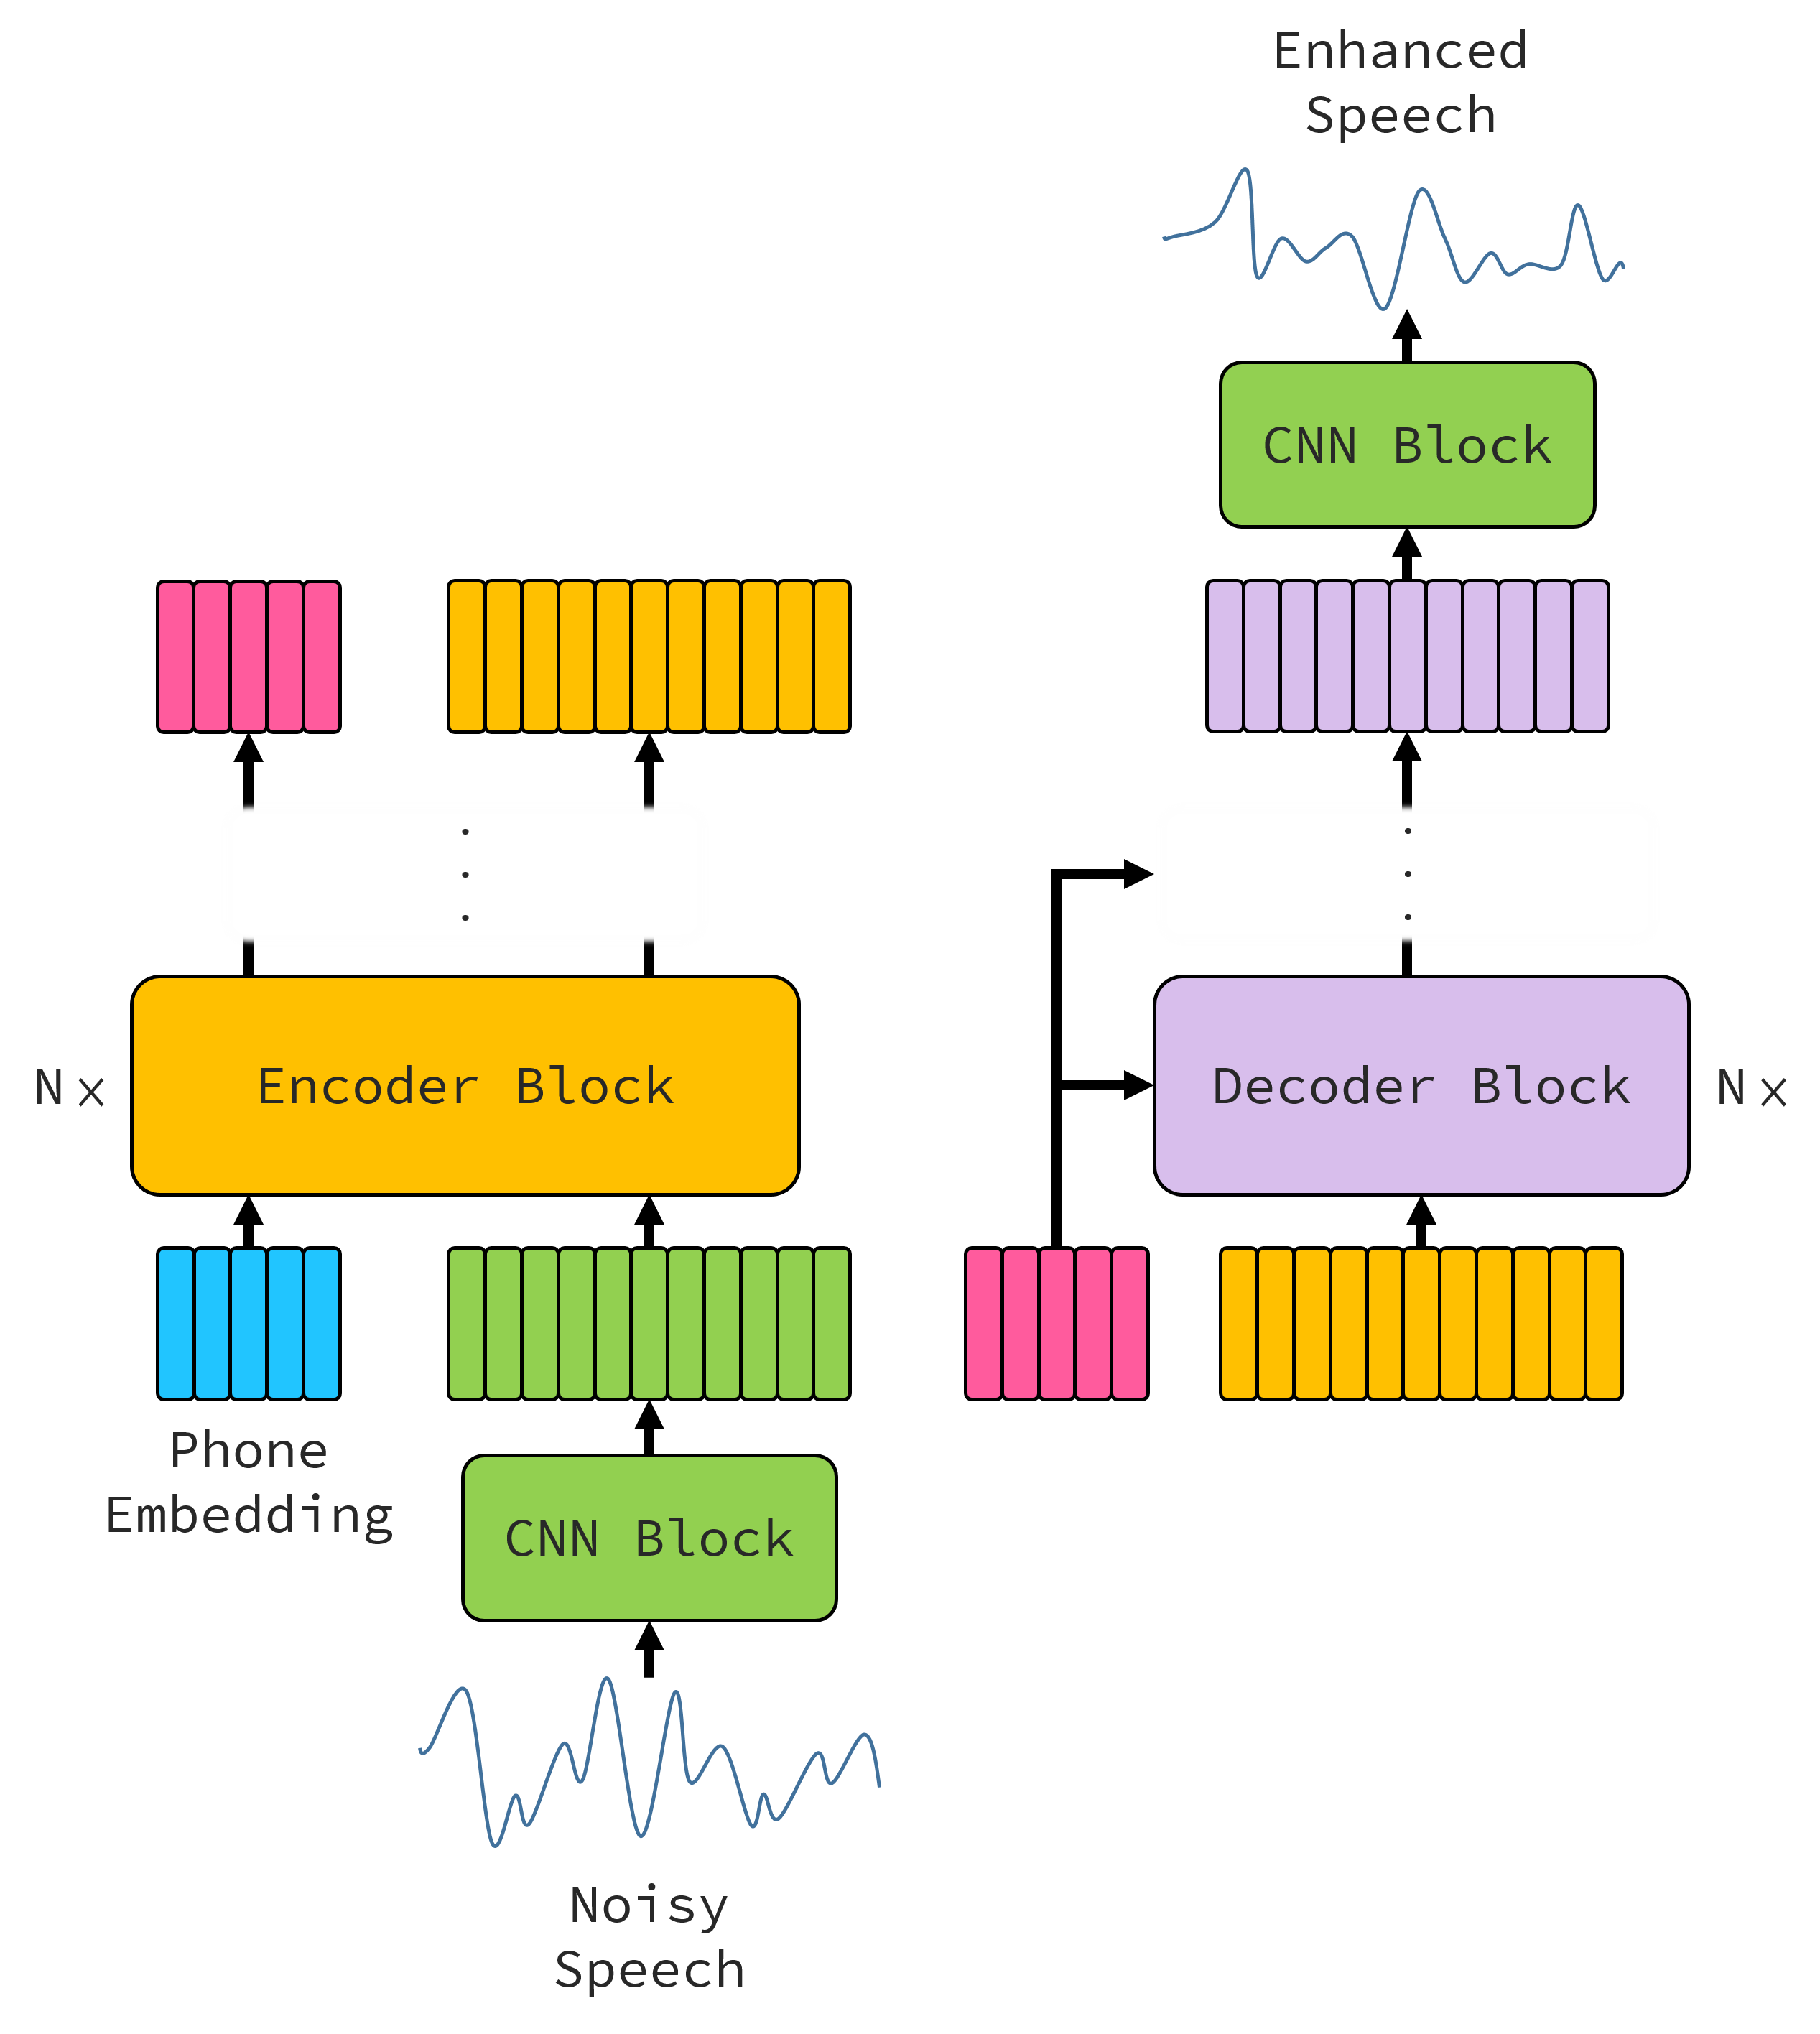
\includegraphics[scale=0.35]{img/architecture.png}
   %    \end{center}
   %    \caption{Example of a short caption, which should be centered.}
   %    \label{fig:short}
   % \end{figure*}



   % \begin{figure*}
   %    \begin{center}
   %       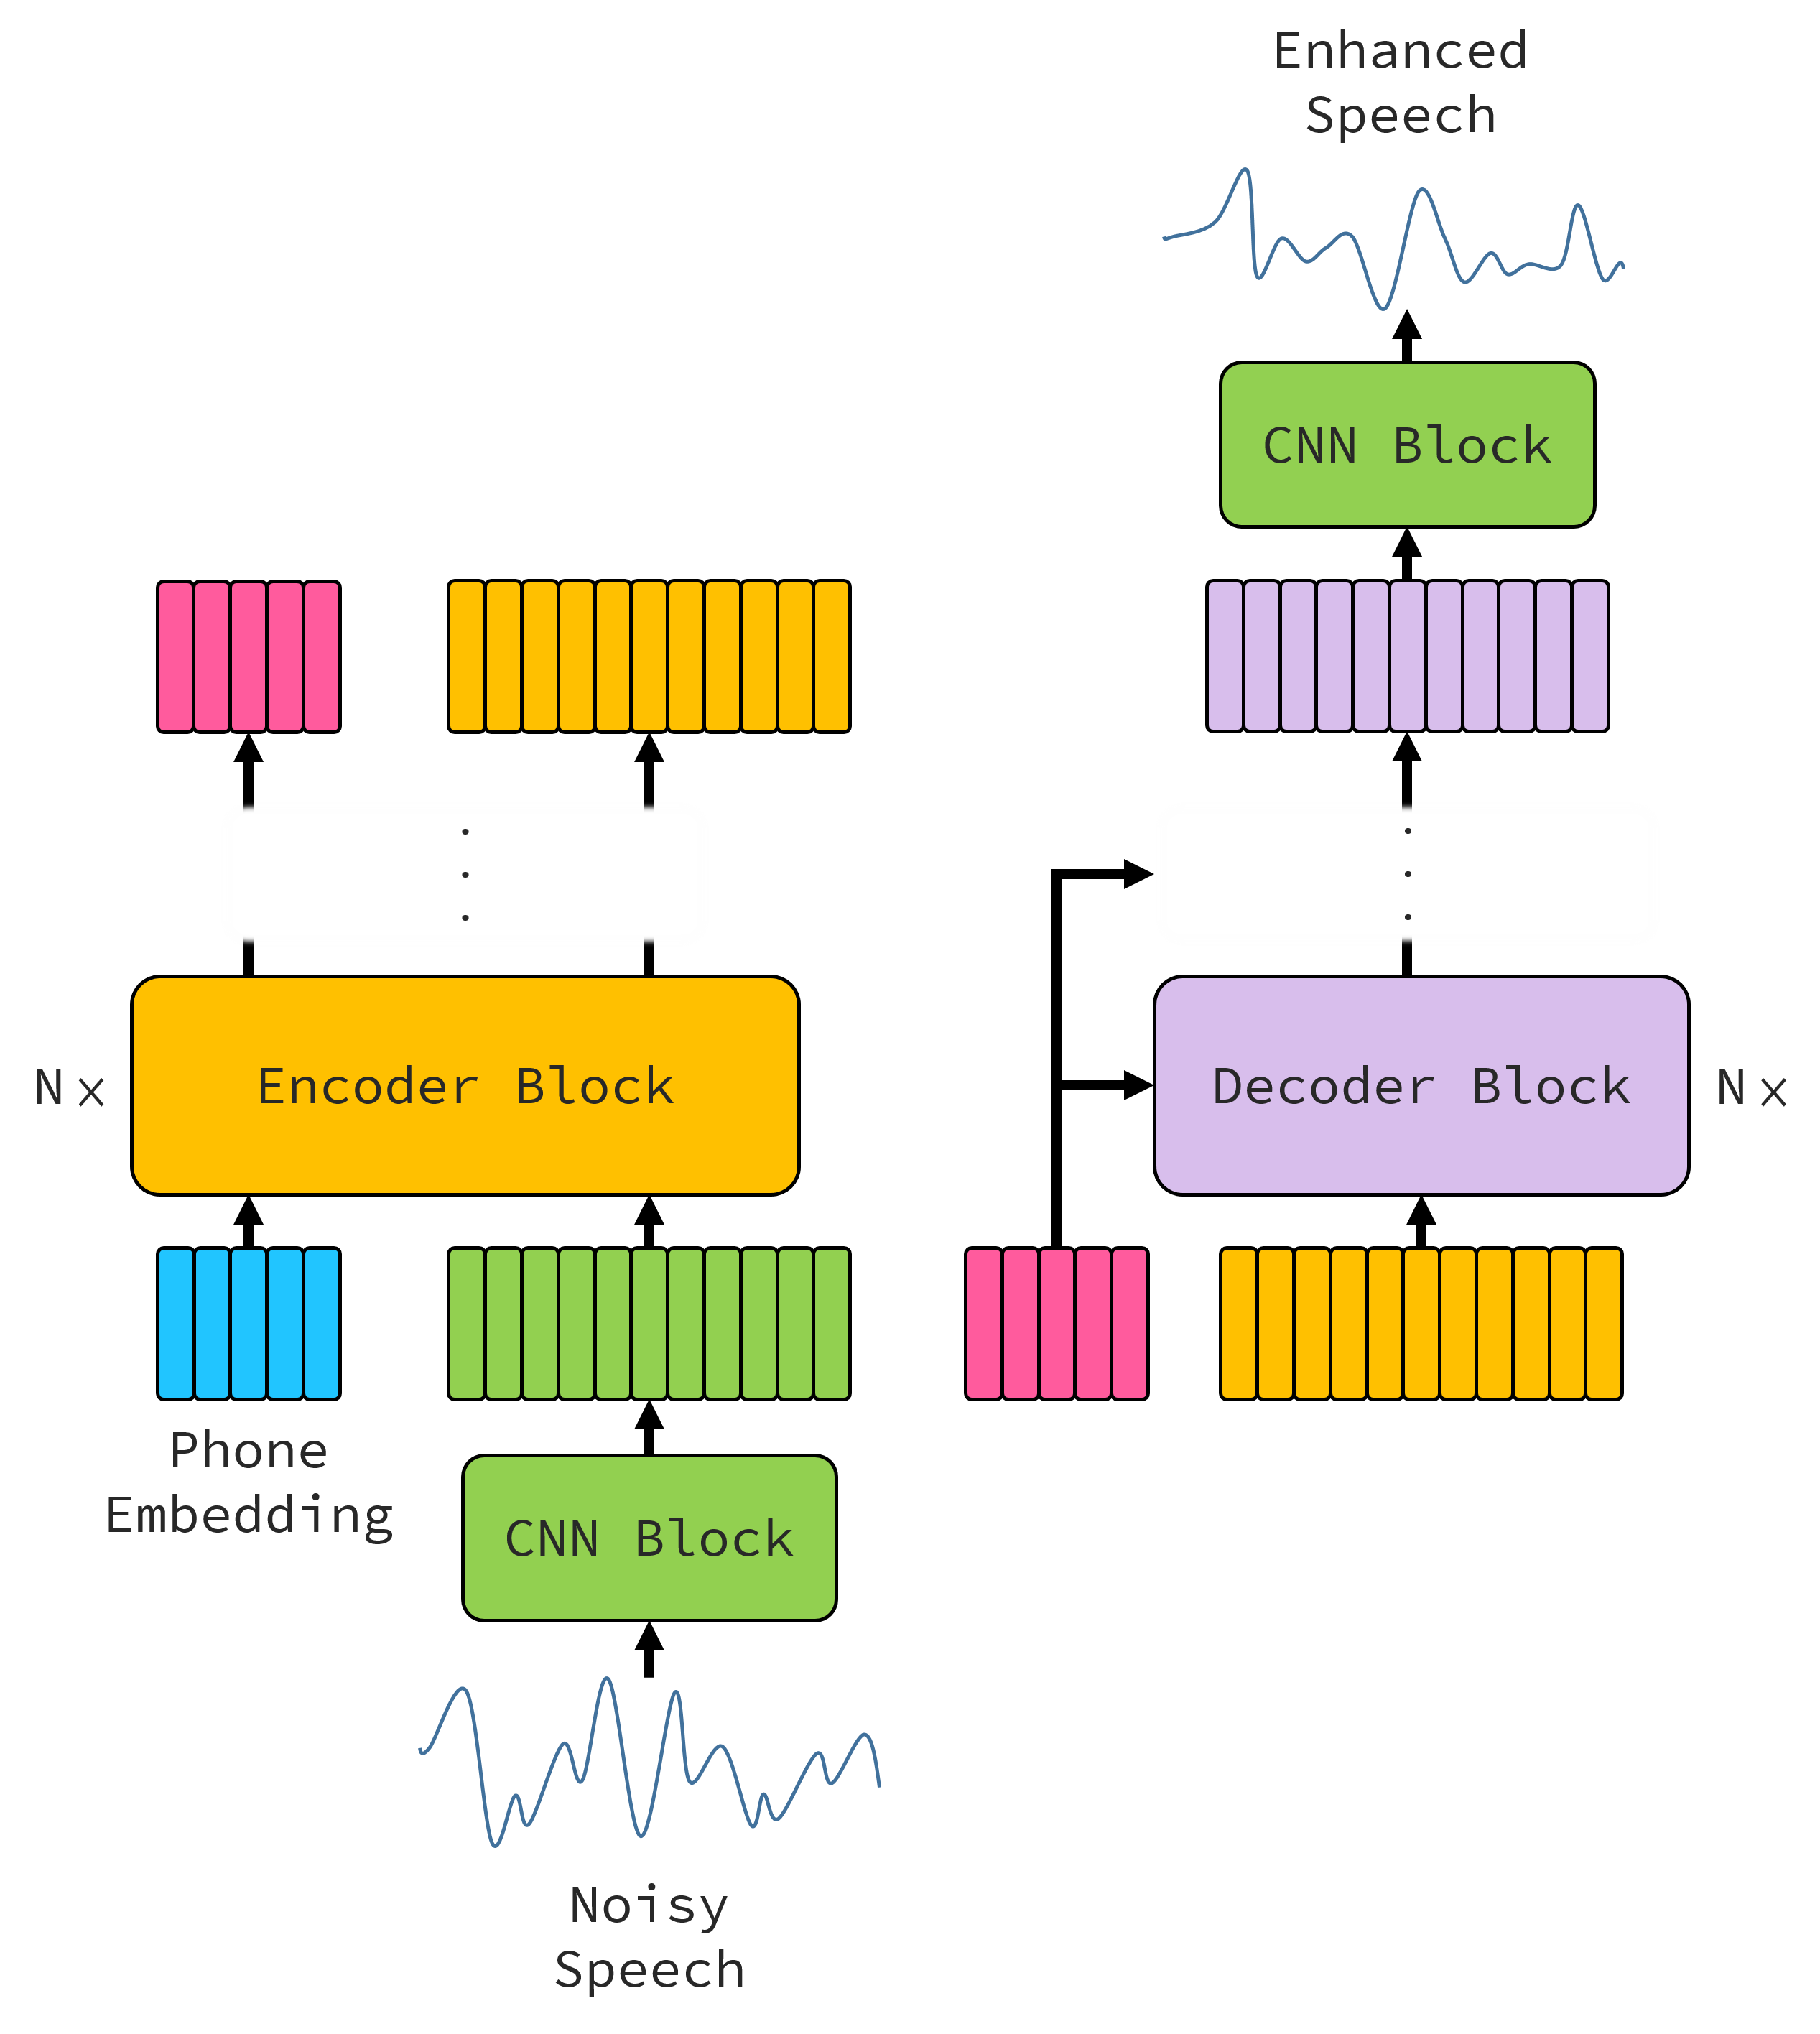
\includegraphics[scale=0.35]{img/architecture.png}

   %    \end{center}
   %    \caption{Example of a short caption, which should be centered.}
   %    \label{fig:short}
   % \end{figure*}
   \begin{figure}[t]
      \begin{center}
         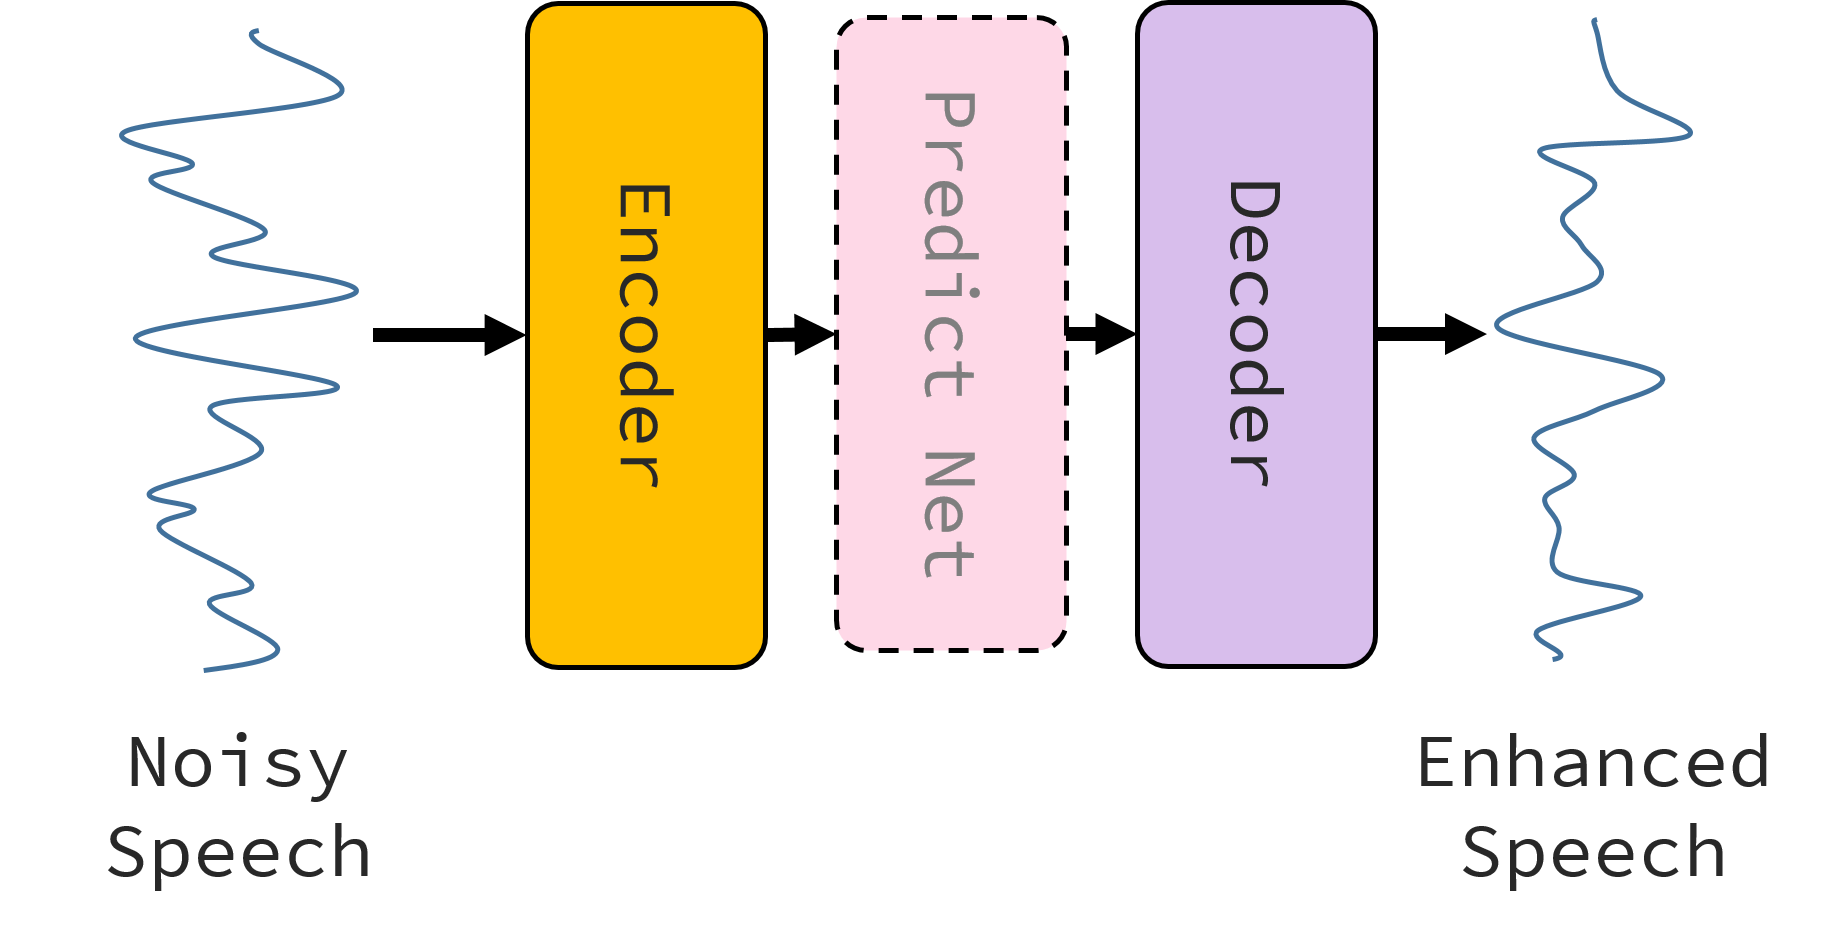
\includegraphics[width=0.8\linewidth]{img/auto-encoder.png}
      \end{center}
      \caption{
         語音增強使用的 Auto Encoder。期望模型能將受雜訊污染的語音還原成乾淨語音。
      }
      \label{fig:long}
      \label{fig:onecol}
   \end{figure}

   \begin{figure}[t]
      \begin{center}
         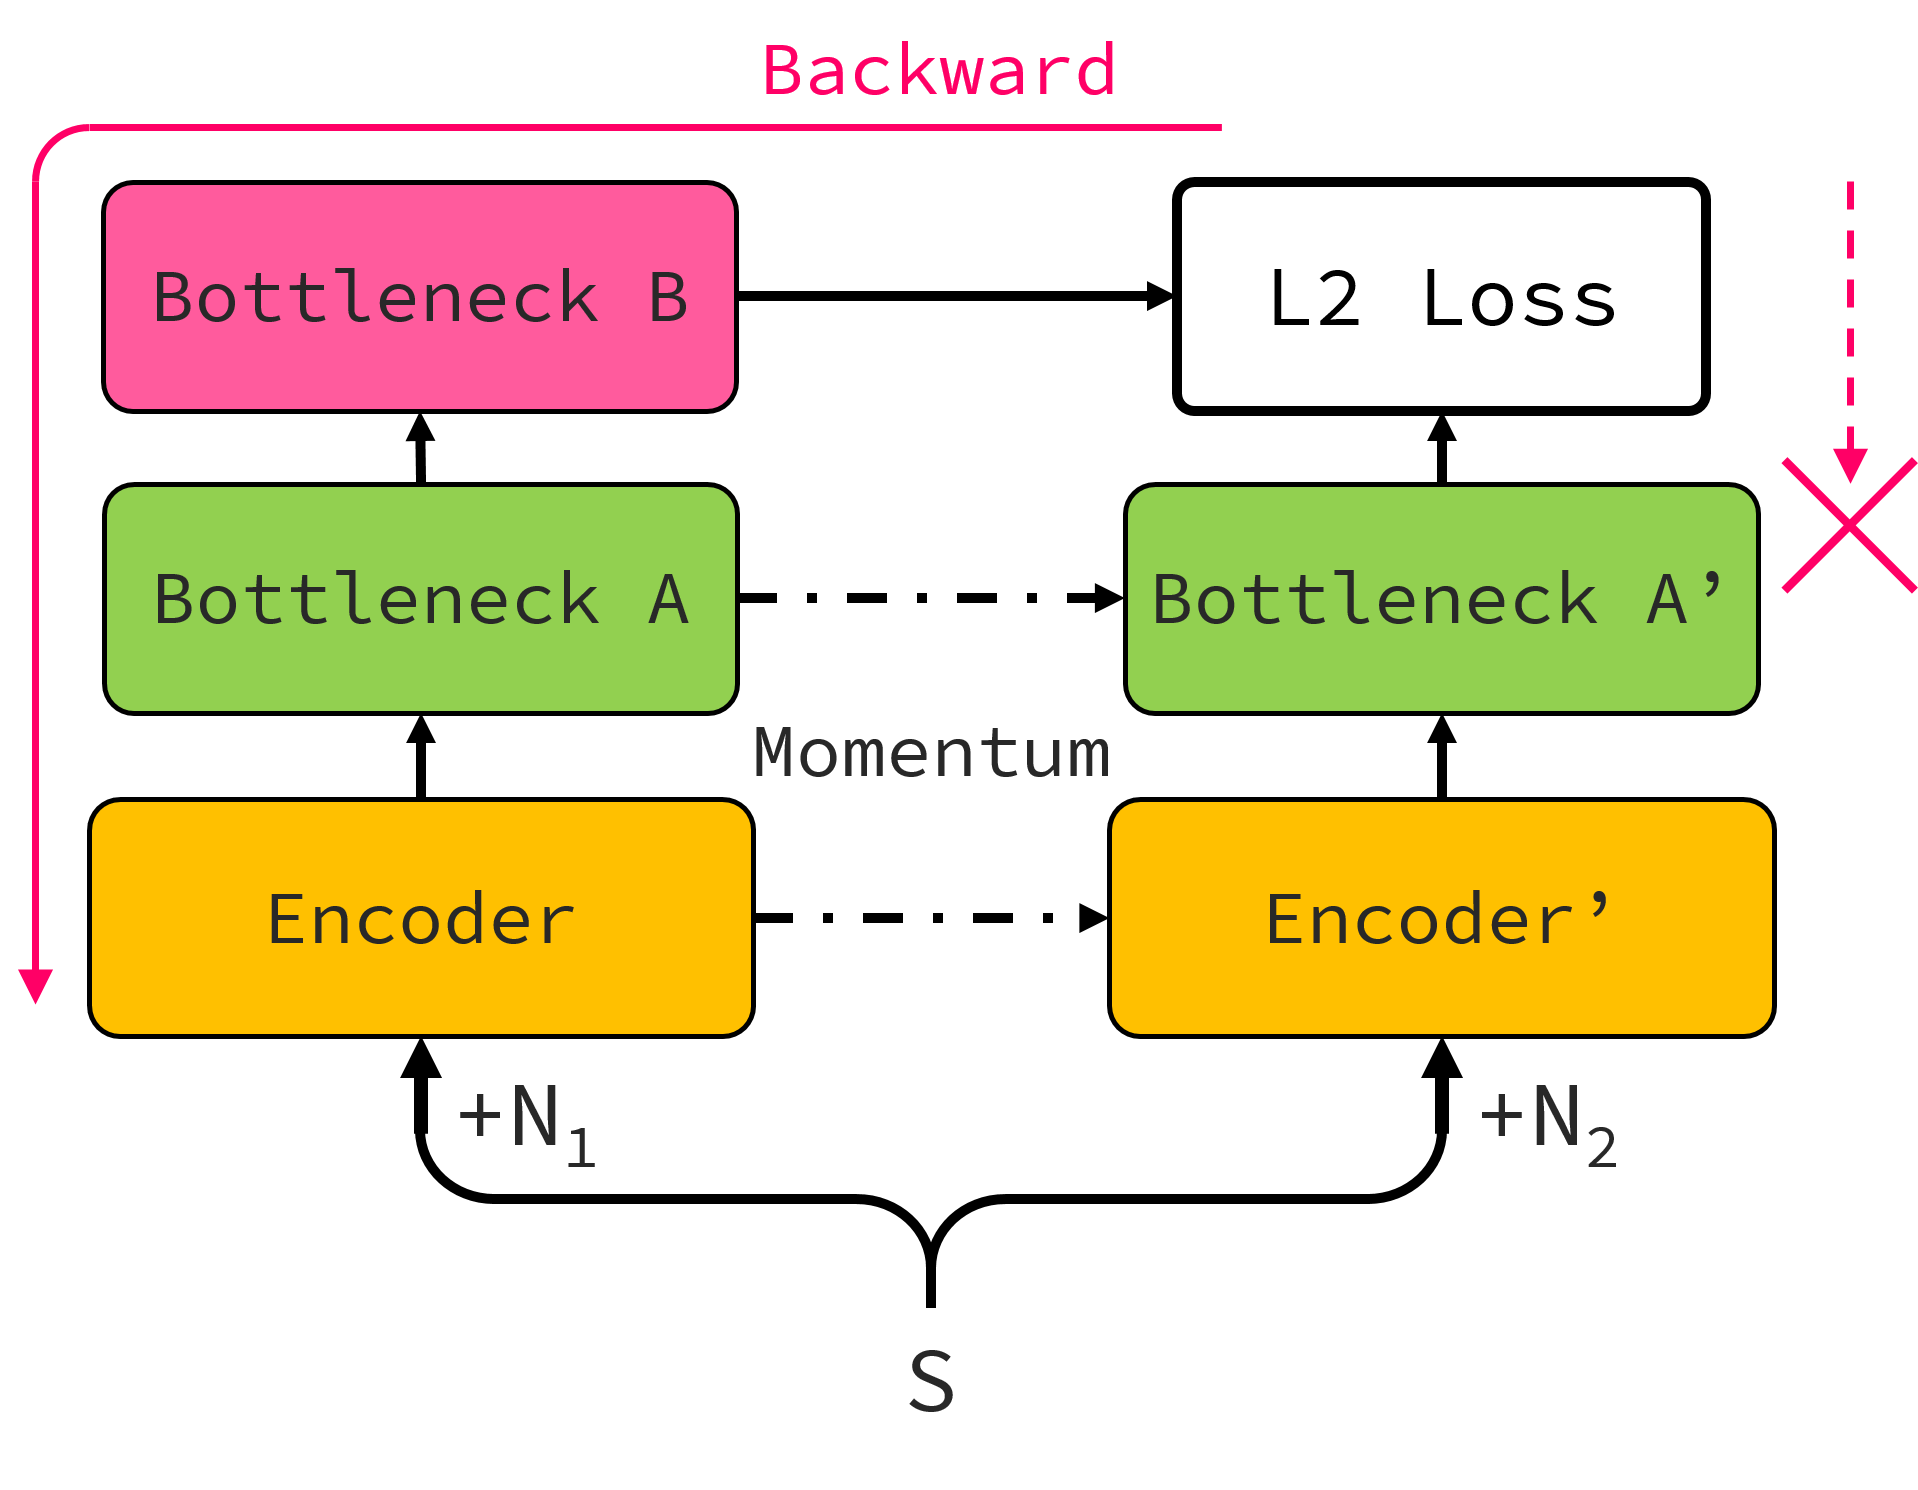
\includegraphics[width=0.8\linewidth]{img/BYOL.png}
      \end{center}
      \caption{
         BYOL 的算法架構。Encoder-PredictNet 會將 Encoder' 取出特徵做為目標,
         計算 L2 Loss 後更新 Encoder-PredictNet 的參數,
         Encoder' 則會把自身目前參數與更新後 Encoder 做加權平均當新參數。
      }
      \label{fig:long}
      \label{fig:onecol}
   \end{figure}

   \begin{figure}[t]
      \begin{center}
         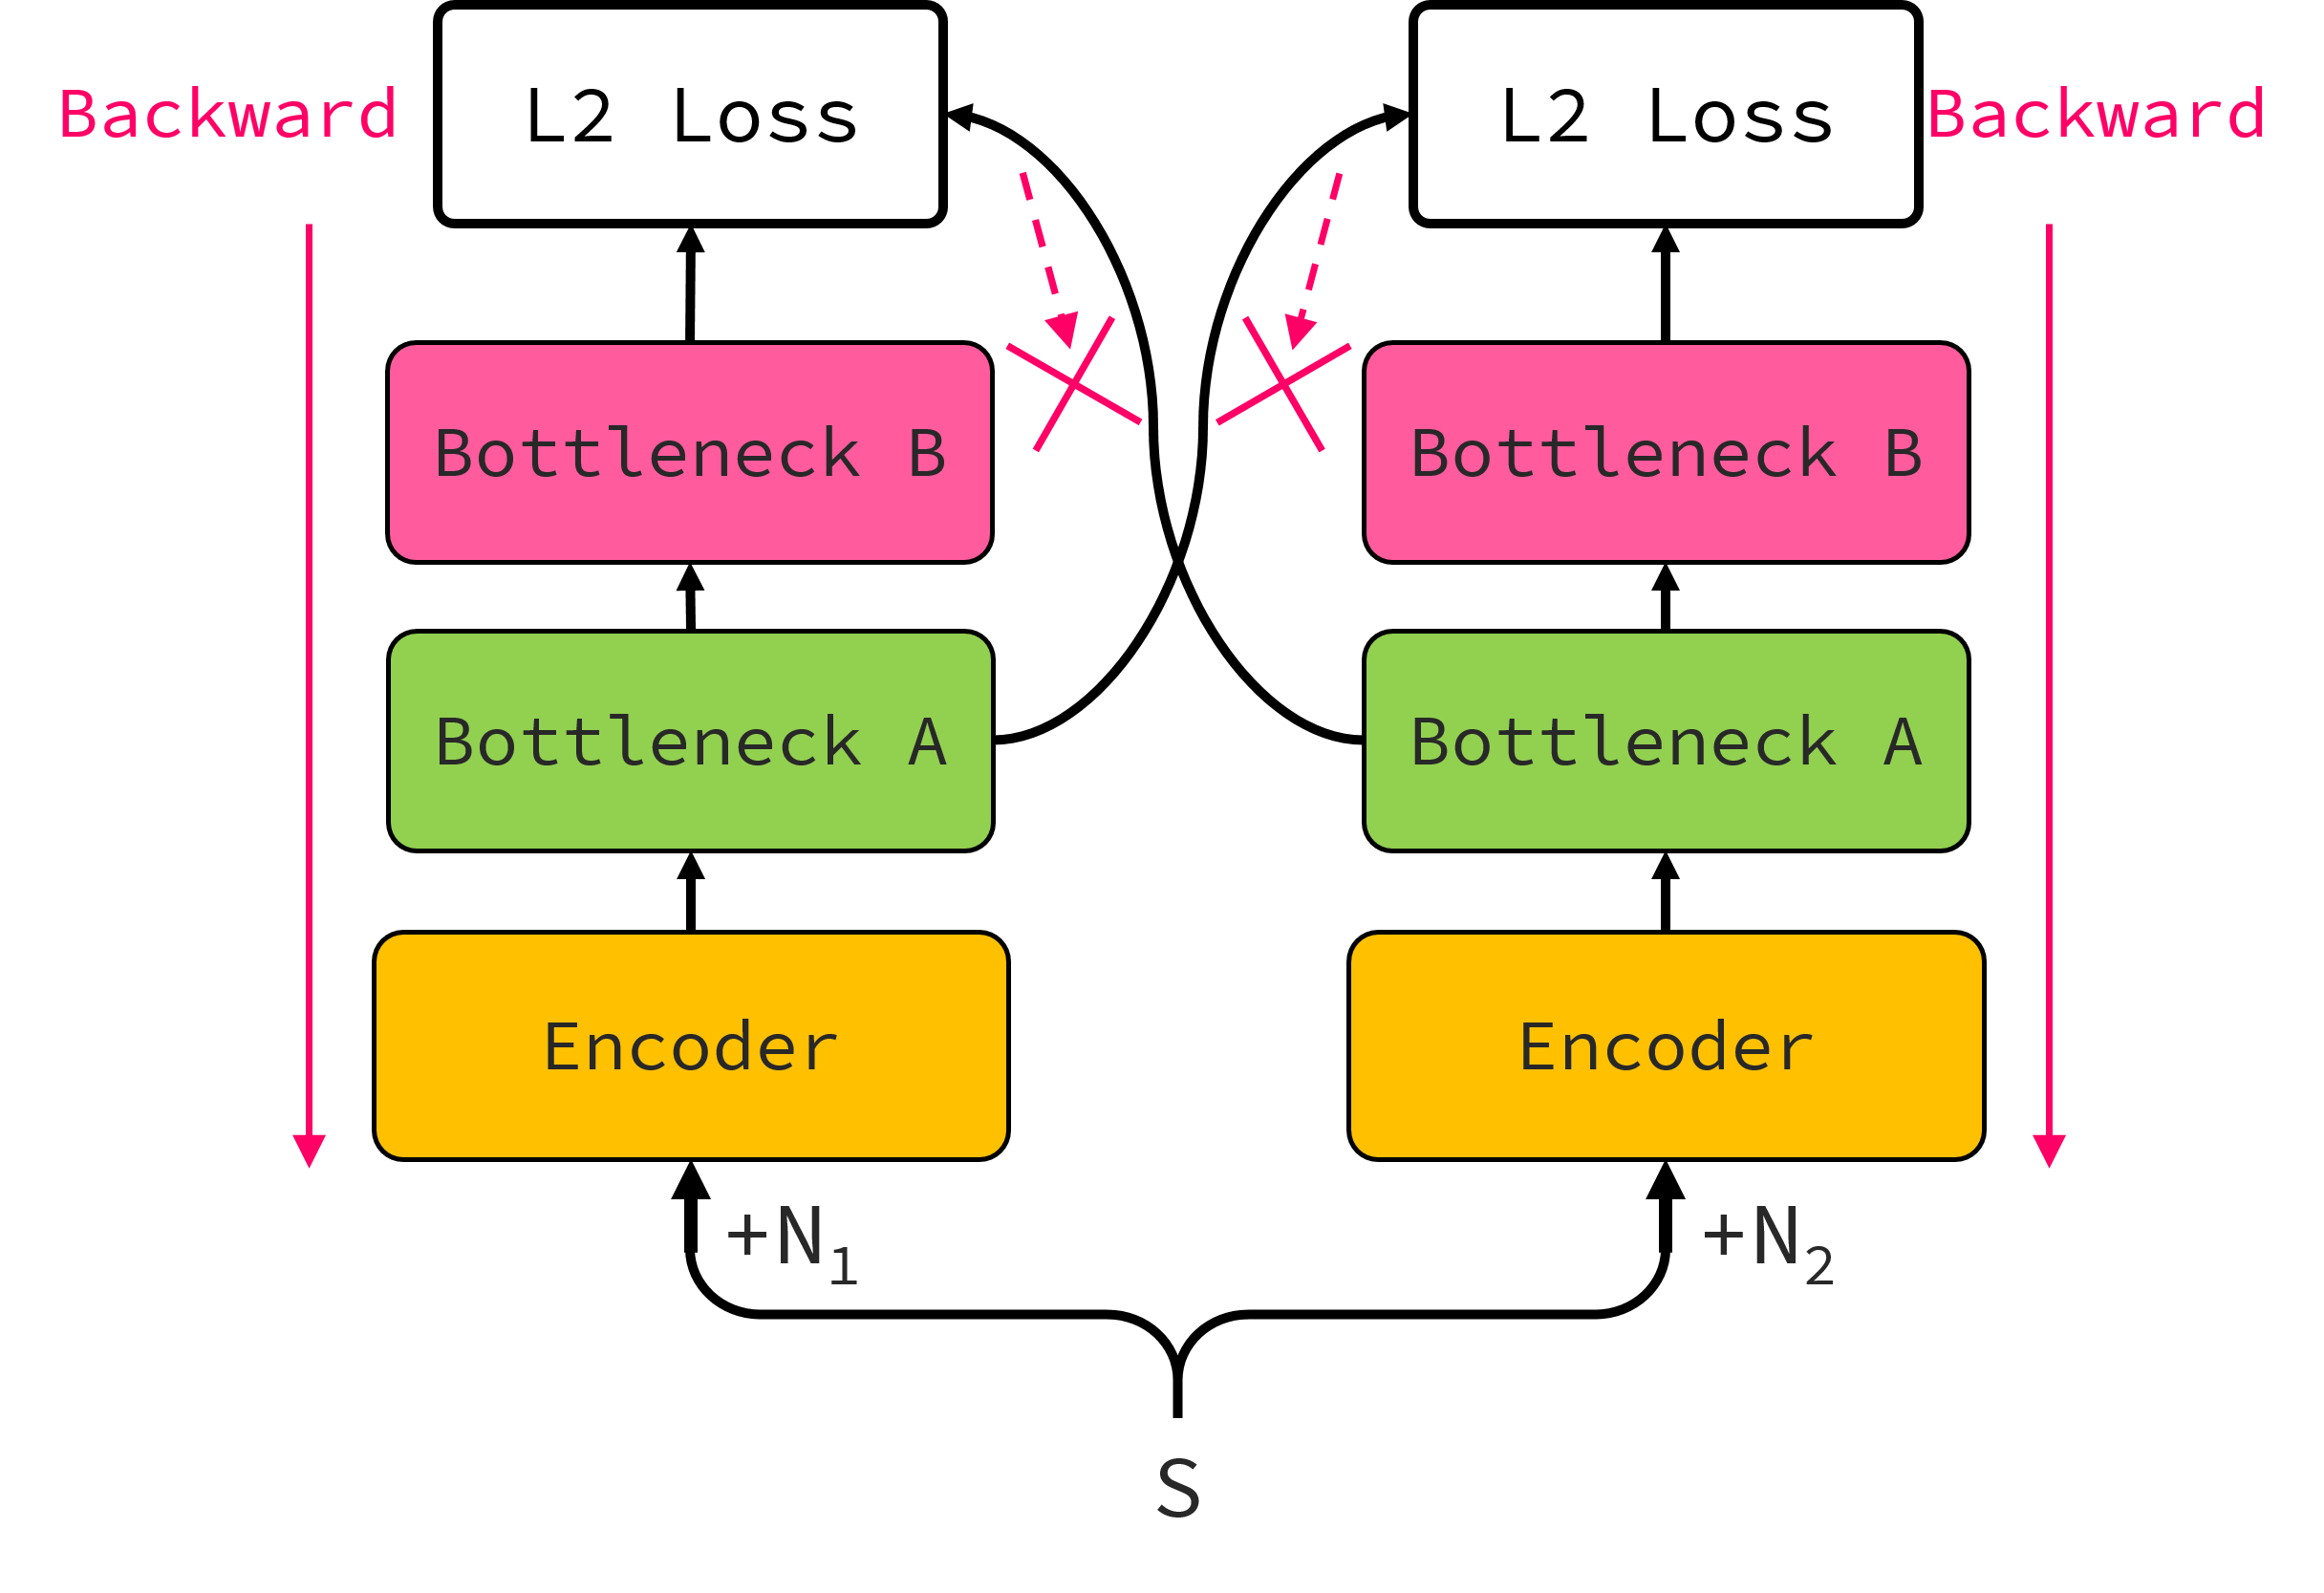
\includegraphics[width=0.8\linewidth]{img/SimSiam.png}
      \end{center}
      \caption{
         SimSiam 的算法架構。將混合不同噪音的語音輸入 Encoder 得到 $Z_1$ 與 $Z_2$,
         在將 $Z_1$ 與 $Z_2$ 輸入 PredictNet 後獲得 $P_1$ 與 $P_2$,
         $P_1$ 與 $P_2$ 會各自將 $Z_2$ 與 $Z_1$ 做為目標並計算差距,
         以此更新 Encoder-PredictNet 的參數。
      }
      \label{fig:long}
      \label{fig:onecol}
   \end{figure}
   %------------------------------------------------------------------------
   \section{System framework}
   本專題使用的模型結構如 Figure 1. 所示,是由 Encoder 與 Decoder 兩區塊組合而成,
   其中負責抽取語音特徵 Encoder 區塊將會使用 BYOL 與 SimSiam 進行預訓練。
   在進行 CL 訓練時,語音 $S$ 會混合 $N_1$ 與 $N_2$ 兩個不同的噪音後,輸入 Encoder
   取出語音的特徵向量,並用 Figure 2. 與 Figure 3. 所述的方法更新其內部權重。

   在使用 CL 預訓練完 Encoder 後,便會將其串接上
   Decoder,將乾淨的語音當成目標來進行語音增強任務的學習。更詳細的實驗內容在 Expected results 中。


   %------------------------------------------------------------------------
   \section{Expected results}
   本專題使用的噪音資料集是由 20 種不同類型的背景噪音所組成,總共有 100 個音檔的 Nonspeech~\cite{Nonspeech}。
   而語音資料集則是選用 TIMIT~\cite{timit},TIMIT 具有 6300 句語音,這些語音包含美國八個地區共 630 人所念出的 10
   個指定句子。在訓練時的噪聲語音是將 TIMIT 與 Nonspeech 以 -5, 0, 5 這三種 SNR 混合產生的。


   % 本專題分別使用 TIMIT~\cite{timit} 與 Nonspeech~\cite{Nonspeech}
   % 作為語音和雜訊的資料集,並以 -5, 0, 5 這三種 SNR 混合成的噪聲語音當模型輸入。
   % Nonspeech 是由 20 種不同類型的背景噪音所組成,總共有 100
   % 個音檔,而 TIMIT 則為 6300 句語音組成資料集,這些語音包含美國八個地區共 630 人所念出的 10
   % 個指定句子。

   本專題預計將會進行以下幾項實驗:
   \begin{enumerate}
      \item 直接對 AutoEncoder 訓練 Speech Enhancement 任務。
      \item 基於 BYOL 對 Encoder 與 Bottleneck 進行預訓練後凍結參數,然後接上 Decoder 訓練 Speech Enhancement 任務。
      \item 基於 SimSiam 對 Encoder 與 Bottleneck 進行預訓練後凍結參數,然後接上 Decoder 訓練 Speech Enhancement 任務。
      \item 將 BYOL 訓練得到的參數作為初始權重後,對 AutoEncoder 訓練 Speech Enhancement 任務。
      \item 將 SimSiam 訓練得到的參數作為初始權重後,對 AutoEncoder 訓練 Speech Enhancement 任務。
      \item 基於不同數量的樣本進行上述實驗,以測試各種方法的泛化能力。
   \end{enumerate}

   最終將比較上述不同方法所訓練得到模型的 PESQ\cite{PESQ}、STOI\cite{STOI} 與 SISDR\cite{SISDR}。


   {\small
   \bibliographystyle{unsrt}
   \bibliography{egbib}
   }
\end{CJK}
\end{document}
